\documentclass{article}
\usepackage{graphicx} % Required for inserting images
\usepackage{amsmath}
\usepackage[a4paper, total={6in, 8in}]{geometry} 
\usepackage{caption}      % For captions
\usepackage{subcaption}   % For subfigures
\usepackage{hyperref}

% references
\usepackage{hyperref}
\usepackage[style=mla]{biblatex}
\addbibresource{sample.bib}

\title{Memory notes}
\author{Simon Thill}
\date{August 2024}

\begin{document}

\maketitle

Code used to make all plots/ diagrams can be found here: \url{https://github.com/Simont12321/Gravitational-memory-thesis.git }.

\section{Recent Changes}

\begin{itemize}
    \item Solved tricky $\phi$ integral and first r integral. 
    \item Did a literature search and believe all other r integrals must be solved numerically. 
    \item finished Ryden textbook
    \item Added figure \ref{fig:BBH energy density per Hz} of gravitational wave energy-density versus wavelength. 
    \item Added an instrumentation section on current CMB telescopes. 
\end{itemize}

\section{Madison's equaitons}

Redshift and angular deflection equations from \cite{madison2021framework} are 

\begin{equation}
    z(t, \theta, \phi) = \frac{h_M}{4}(e^{2i\phi} + e^{-2i\phi})(1-\cos\theta)\Theta(\theta_t - \theta)
    \label{eq: z_madison}
\end{equation}

where $\cos(\theta_t) = \beta - 1$, and $\beta = ct/d$ where $d$ is the distance to the light source being redshifted. $\theta_t$ is therefore a cutoff angle for redshift perturbations. 


\begin{equation}
    \delta\vec{n}(t,\hat{n}) = h_M \{\vec{V}_\oplus(\hat{n}) - \vec{V}_\star(\hat{n})\left[\frac{\beta\Theta(\theta_t - \theta)}{(1+\cos\theta)} + \Theta(\theta - \theta_t)\right]\}
    \label{eq: del_n_madison}
\end{equation}

where 

\begin{equation}
    \vec{V}_\oplus = -\frac{1}{4}\sin\theta \left[(e^{2i\phi} + e^{-2i\phi})\hat{\theta} + i(e^{2i\phi} - e^{-2i\phi})\hat{\phi}\right], 
    \label{eq: V_earth_madison}
\end{equation}
and 
\begin{equation}
    \vec{V}_\star = -\frac{1}{4}\sin\theta \left[(1+\cos\theta)(e^{2i\phi} + e^{-2i\phi})\hat{\theta} + 2i(e^{2i\phi} - e^{-2i\phi})\hat{\phi}\right]
    \label{eq: V_star_madison}
\end{equation}

\section{Flat-sky approximation}

\subsection{Useful formulas}
Taylor series:

\begin{equation*}
    \cos(x) \approx 1 - \frac{x^2}{2} + \frac{x^4}{24}
\end{equation*}

\begin{equation*}
    \sin(x) \approx x - \frac{x^3}{6} + \frac{x^5}{120}
\end{equation*}

Euler's formula:

\begin{equation*}
    e^{ix} = \cos(x) + i\sin(x) 
\end{equation*}

In the flat-sky approximation, a small change in angle $d\theta$ is taken to be equal to a change in Cartesian coordinates $d\theta_y$ where $d\theta_y = \frac{dy}{r}$. Similarly $d\phi = d\theta_x = \frac{dx}{r}$ where $r$ is the radial distance in polar coordinates.
\\

\subsection{Redshift}
Substituting $(\theta, \phi) \rightarrow (\theta_y, \theta_x)$, using Euler's formula, and Taylor expanding equation \ref{eq: z_madison} gives

\begin{align}
    z(t,y,x) &\rightarrow \frac{h_M}{4} 2\cos(2x)(1-\cos(y))\Theta(y_t - y) \notag \\
    &\approx \frac{h_M}{2}(1-2x^2)(1-1-\frac{y^2}{2})\Theta(y_t - y) \notag \\ 
    &= \frac{h_M}{2}(-\frac{y^2}{2} + x^2y^2)\Theta(y_t - y) \label{eq:z_flatsky}
\end{align}

For simplicity, I have used $(x,y)$ rather than $(\theta_y, \theta_x)$. The initial redshift is plotted in this flat-sky approximation in figure \ref{fig:redshift} which matches up well with Madison's full equation \ref{eq: z_madison} plotted in figure \ref{fig:redshift_madison}. Madison's full equaiton is also plotted in polar coordinates in figure \ref{fig:polar_z_madison}. 
\\

This equation is centered on the Earth's pole. A more general expression for  any location where $x \rightarrow x+\Delta x$ and $y \rightarrow y+\Delta y$ is graphed in figure \ref{fig:z_displaced} and given by the equation 

\begin{equation}
    z(t,y,x) = \frac{-h_M}{4}(y^2 +y\Delta y + \Delta y^2) + \frac{h_M}{2}(x^2 +x\Delta x + \Delta x^2)(y^2 +y\Delta y + \Delta y^2).
\end{equation}

\begin{figure}
    \centering
    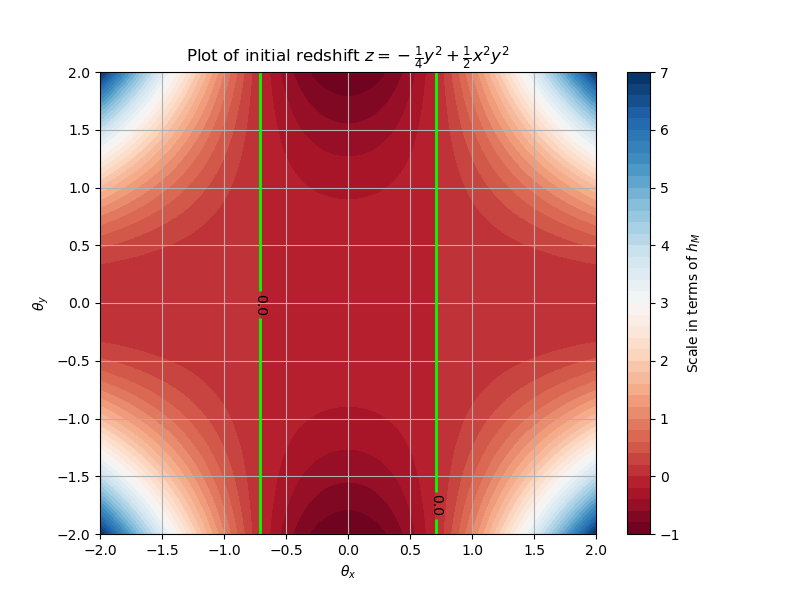
\includegraphics[width=0.7\linewidth]{figures/redshift.png}
    \caption{Plot of initial flat-sky redshift given by equation \ref{eq:z_flatsky}. As it is the initial perterbation there is no cut-off angle. The 0-redshift contour is highlighted.}
    \label{fig:redshift}
\end{figure}


\begin{figure}
    \centering
    \begin{subfigure}[b]{0.45\textwidth}
        \centering
        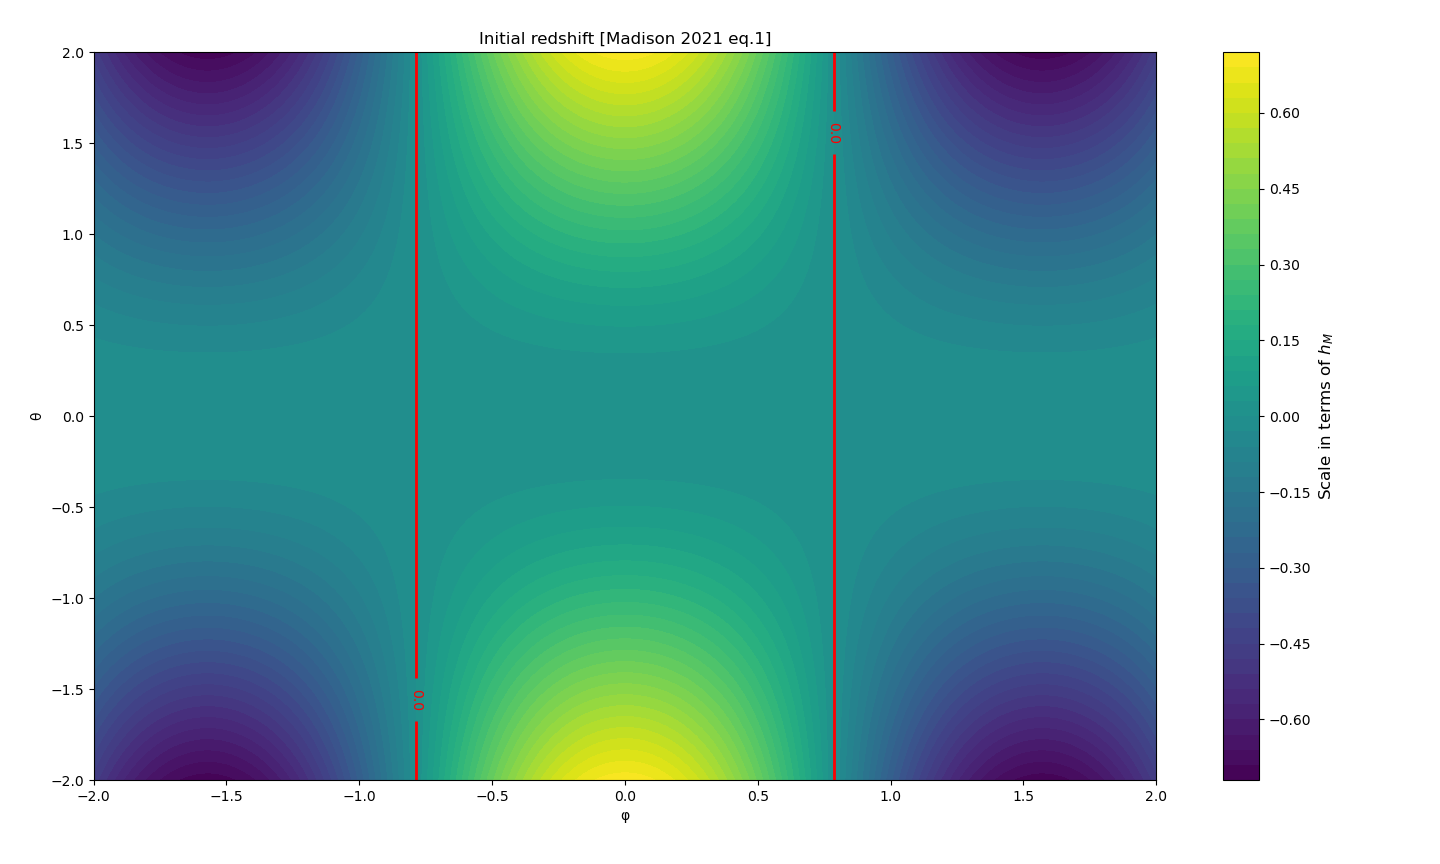
\includegraphics[width=\textwidth]{figures/z_madison.png}
        \caption{Madison's redshift equation [\ref{eq: z_madison}] plotted over the same range as figure \ref{fig:redshift} with contour lines at z = 0.} 
        \label{fig:redshift_madison}
    \end{subfigure}
    \hfill 
    \centering
    \begin{subfigure}[b]{0.45\textwidth}
        \centering
        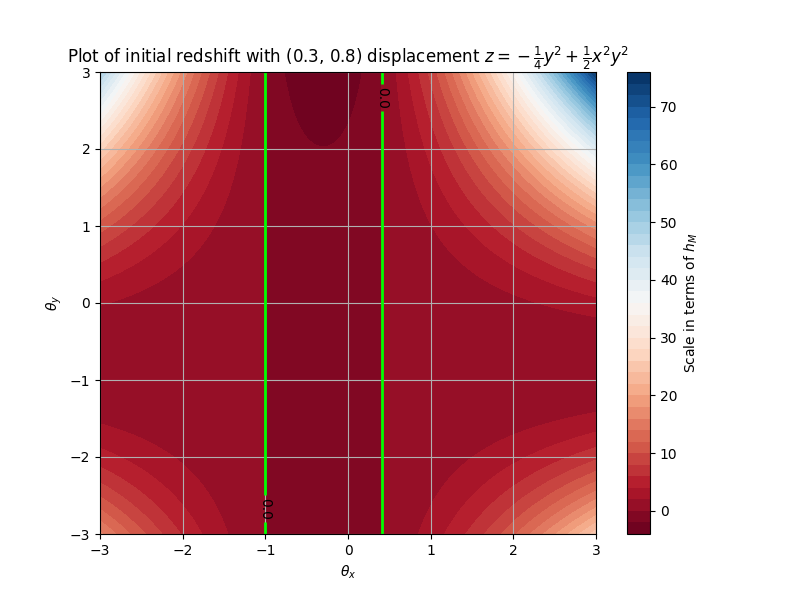
\includegraphics[width=\textwidth]{figures/z_displaced.png}
    \caption{Initial flat-sky redshift not centered on the South Pole.}
    \label{fig:z_displaced}
    \end{subfigure}
\end{figure}

\begin{figure}
    \centering
    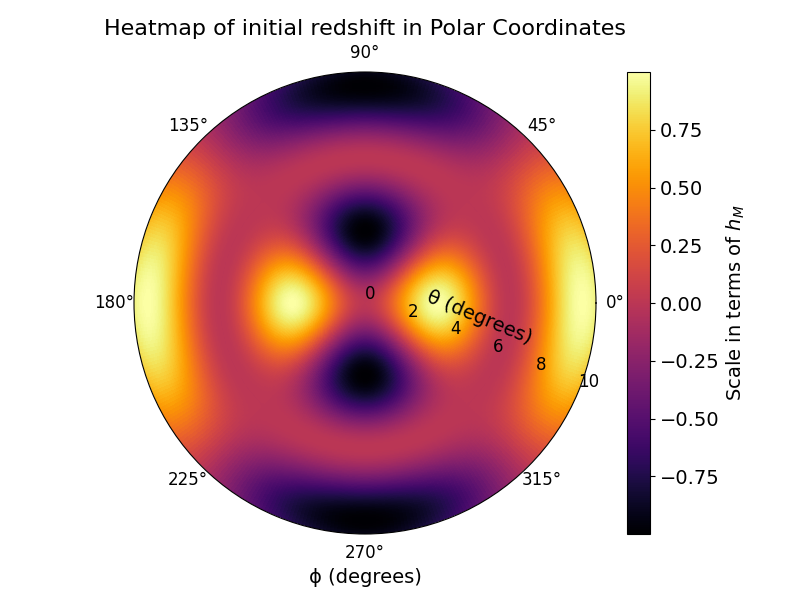
\includegraphics[width=0.5\linewidth]{figures/full_z_madison.png}
    \caption{Initial redshift $z(t=0, \theta, \phi$)}
    \label{fig:polar_z_madison}
\end{figure}

\subsection{Deflection angle}
Substituting $(\theta, \phi) \rightarrow (\theta_y, \theta_x)$, using Euler's formula, and Taylor expanding equation \ref{eq: del_n_madison} gives


\begin{equation}
    \delta\vec{n}(t,\hat{n}) \rightarrow h_M \{\vec{V}_\oplus - \vec{V}_\star\left[\frac{\beta\Theta(y_t - y)}{1+\cos(y)} + \Theta(y-y_t)\right]. 
    \label{eq:dn flatsky subs}
\end{equation}

Working through $\vec{V}_\oplus$ and $\vec{V}_\star$ individually and dropping any terms larger than $O(2)$ leads to

\begin{align}
    \vec{V}_\oplus &= -\frac{1}{4}\sin(y)\left[(2\cos(2x)\hat{y} - 2\sin(2x)\hat{x}\right] \notag \\
    &\approx -\frac{1}{4}y[(2-4x^2)\hat{y} - 4x\hat{x}] \notag \\
    &\rightarrow -\frac{1}{2}y\hat{y} + xy\hat{x}, 
    \label{eq:Vearth flatsky subs}
\end{align}

\begin{align}
    \vec{V}_\star &= \left[-\frac{1}{2}\sin(y)\cos(2x)\hat{y} + \sin(y)\sin(2x)\hat{x} - \frac{1}{2} \sin(y)\cos(y)\cos(2x)\hat{y}\right] \notag \\
    &\approx -\frac{1}{2}(1-2x^2)\hat{y} + 2xy\hat{x} - \frac{1}{2}y(1-\frac{y^2}{2})(1-2x^2)\hat{y}) \notag \\
    &\rightarrow \frac{1}{2}y\hat{y} - x^2y\hat{y} - 2xy\hat{x} +\frac{1}{2}y(1-2x^2-\frac{y^2}{2})\hat{y} \notag \\
    &\rightarrow y\hat{y} - 2xy\hat{x}.
    \label{eq:Vstar flatsky subs}
\end{align}

If $y > y_t$ there is no more time-variation and $\delta\vec{n}$ has reached it's final value. Substituting equations \ref{eq:Vearth flatsky subs} and \ref{eq:Vstar flatsky subs} into \ref{eq:dn flatsky subs} gives the final deflection angle 

\begin{equation}
    \delta\vec{n}(t\rightarrow\infty,\hat{n}) = h_M[-xy\hat{x} + \frac{1}{2}y\hat{y}].
    \label{eq: final flatsky deflection}
\end{equation}

However, if $y_t > y$, the deflection has some time dependence given by $\beta = ct/d$ and 

\begin{align}
    \delta\vec{n}(t,\hat{n}) &= h_M[xy\hat{x} - \frac{1}{2}y\hat{y} + \frac{\beta}{2}[y\hat{y}  - 2xy\hat{x}]] \notag \\
    &= h_M[(xy-\beta*xy)\hat{x} + (\frac{-1}{2}y + \frac{\beta}{2}y)\hat{y}] 
    \label{eq: flatsky deflection txy}
\end{align}

which for clarity can also be written as the initial deflection plus a time-varying component 
\begin{equation}
    \delta\vec{n}(t,\hat{n}) = h_M[(-xy\hat{x} + \frac{1}{2}y\hat{y})\beta + (xy\hat{x} - \frac{1}{2}y\hat{y})]. 
    \label{eq: flatsky deflection t/B/initial}
\end{equation}

This drops all terms higher than $O(2)$, the next highest term is of order $x^2y$. Equation \ref{eq: flatsky deflection t/B/initial} is centered on the South Pole, but can be written for any general location where $x \rightarrow x+\Delta x$ and $y \rightarrow y+\Delta y$ is graphed in figure \ref{fig:dn_cood_translation} and given by 

\begin{equation}
    \Rightarrow h_M\left\{\left[-(x+\Delta x)(y+\Delta y)\hat{x} + \frac{1}{2}(y+\Delta y)\hat{y}\right]\beta + \left[(x+\Delta x)(y+\Delta y)\hat{x} - \frac{1}{2}(y+\Delta y)\hat{y}\right]\right\}. 
    \label{eq: flatsky deflection cood translation}
\end{equation}
\\

The maximum value of $\beta$ is 2, so in the large t limit the time varying deflection [eq: \ref{eq: flatsky deflection t/B/initial}] equals the final deflection [eq: \ref{eq: final flatsky deflection}]. %The final deflection vectors are shown in figure \ref{fig:dn B=2}. There are null-vectors along the four axes corresponding to the four non-oscillatory points in space for a purely polarized gravitational wave. 

\begin{figure}[htbp]
    \centering
    \begin{subfigure}{0.49\textwidth}
        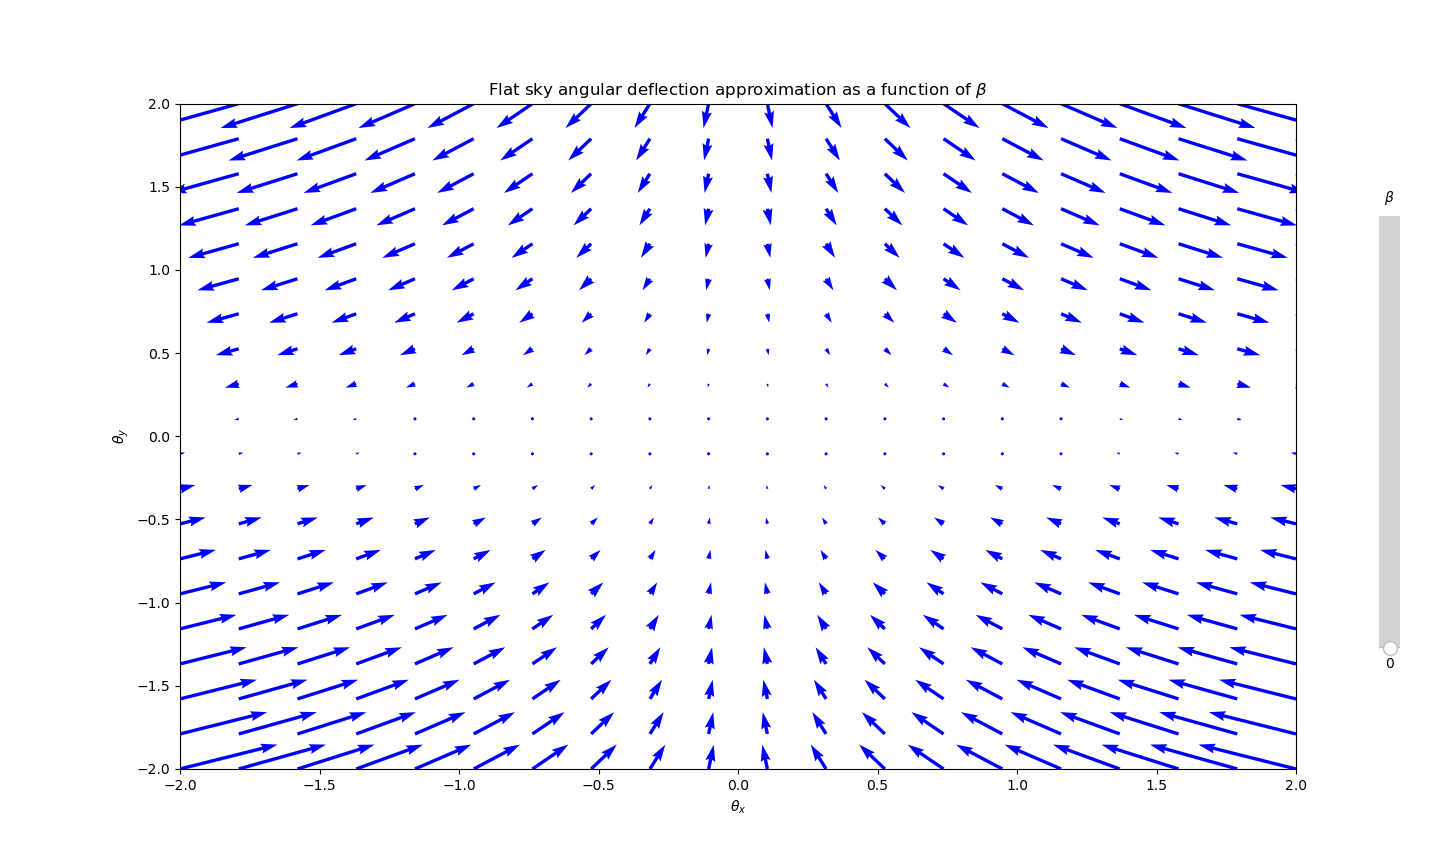
\includegraphics[width=\linewidth]{figures/dn_B0.png}
        \caption{$\beta = 0$, initial deflection.}
        \label{fig:dn B=0}
    \end{subfigure}
    \hfill
    \begin{subfigure}{0.49\textwidth}
        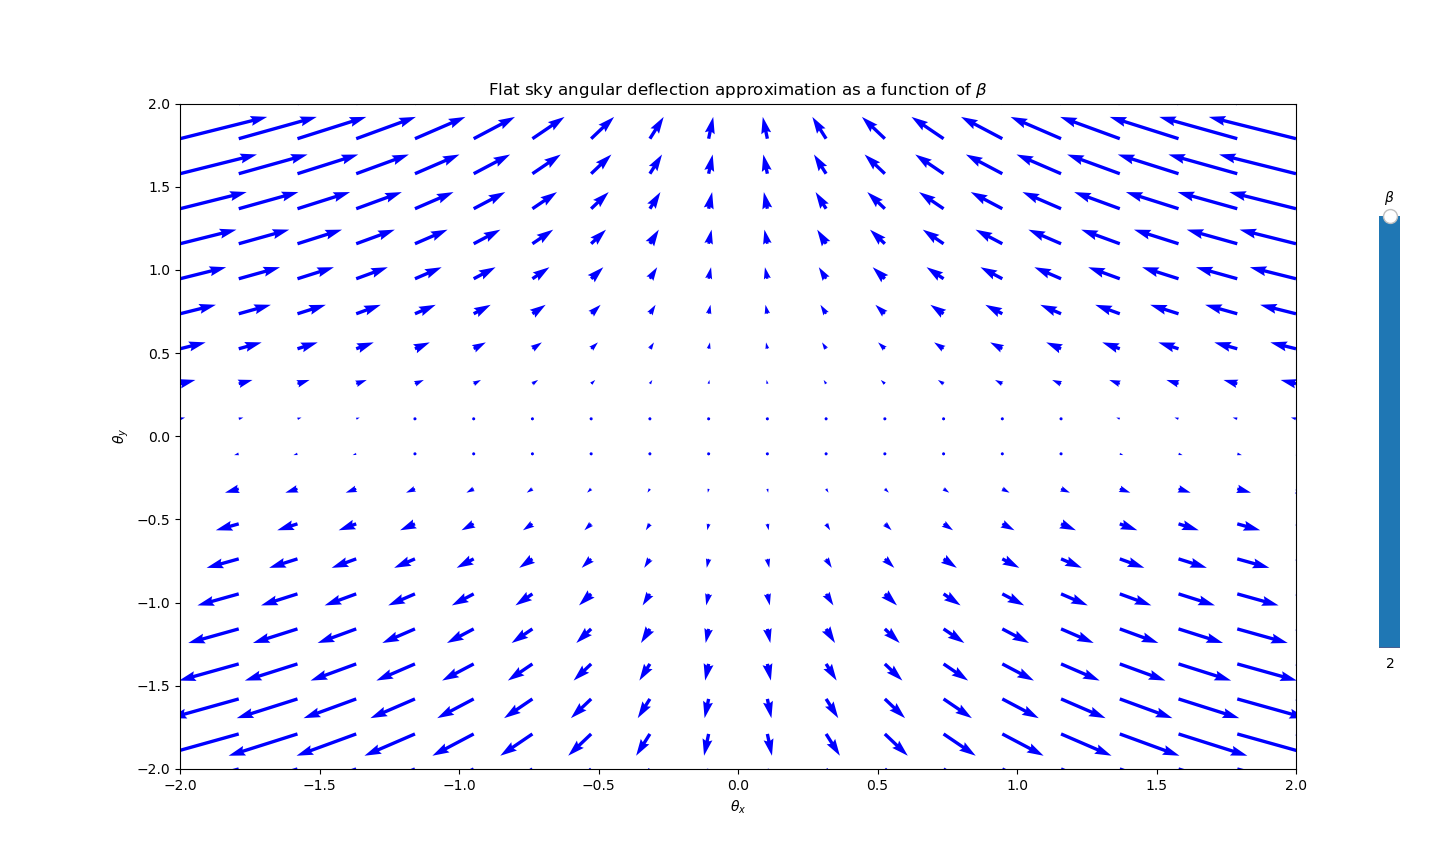
\includegraphics[width=\linewidth]{figures/dn_B2.png}
        \caption{$\beta = 2$, final deflection is equal and opposite to the initial deflection.}
        \label{fig:dn B=2}
    \end{subfigure}
    \vspace{1em}  % Add vertical space between rows
    \begin{subfigure}{0.49\textwidth}
        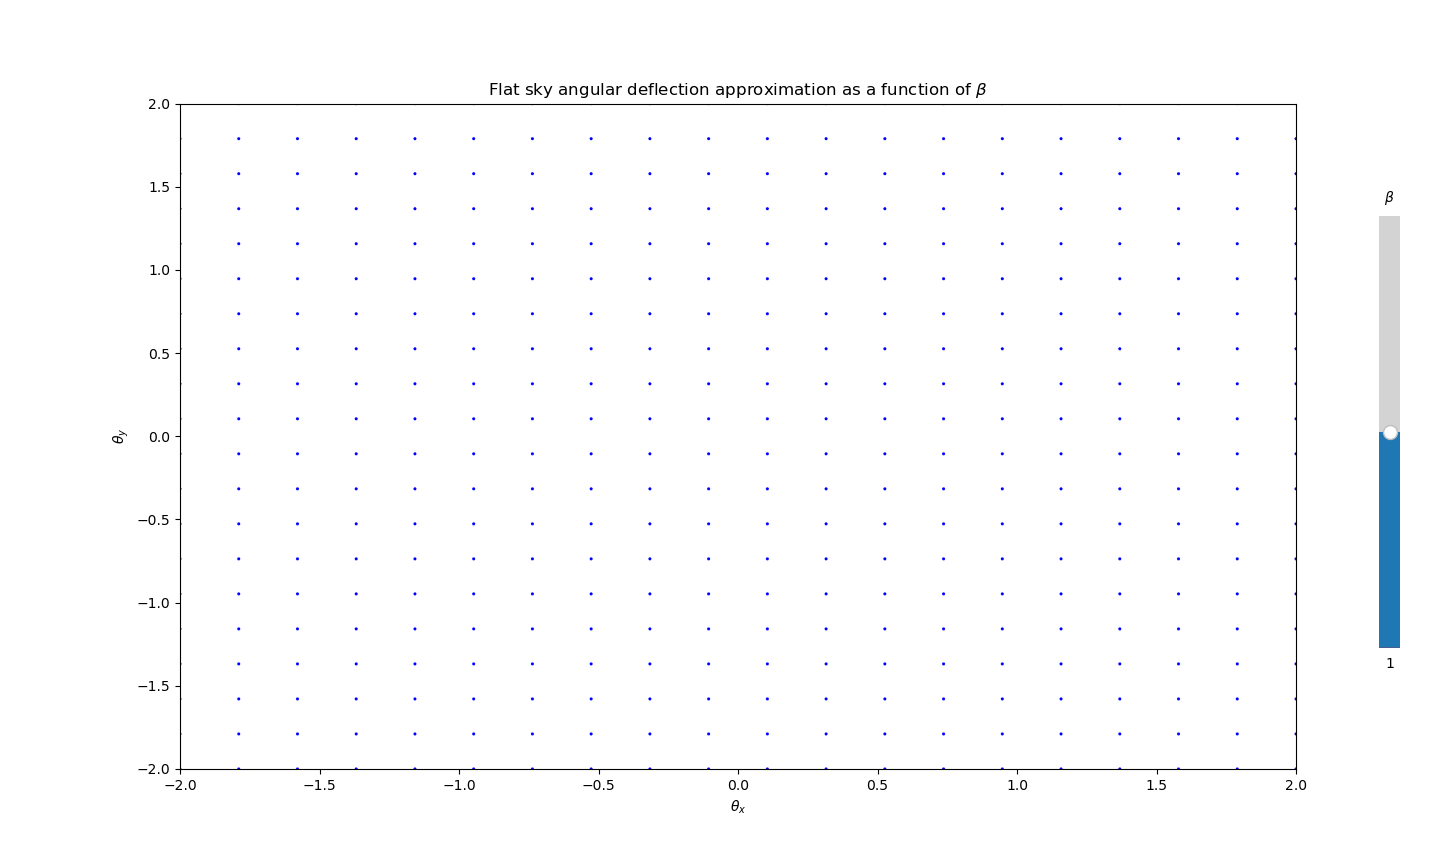
\includegraphics[width=\linewidth]{figures/dn_B1.png}
        \caption{$\beta = 1$, deflection is at its minimum value which is only 0 for a small region about the gravitational wave's propagation vector.}
        \label{fig:dn B=1}
    \end{subfigure}
    \hfill
    \begin{subfigure}{0.49\textwidth}
        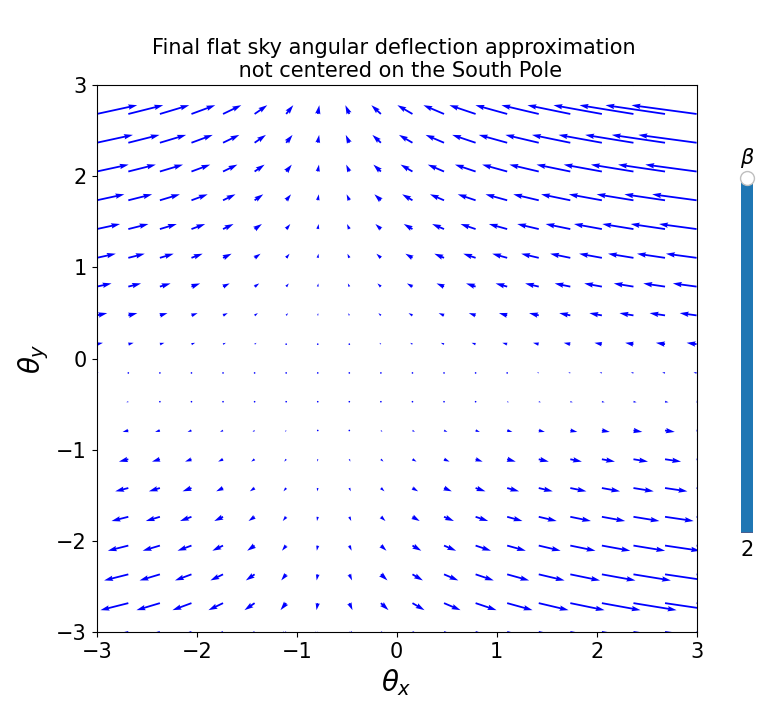
\includegraphics[width=\linewidth]{figures/dn_cood_translation.png}
        \caption{Final deflections not centered on the South Pole.}
        \label{fig:dn_cood_translation}
    \end{subfigure}
    \caption{Angular deflection vector graphs for various values of $\beta$, ranging from 0 to its maximum value of 2.}
    \label{fig:dn_mainfigure}
\end{figure}

\section{Effect on CMB statistics}
From \cite{madison2021framework}, the full expression of CMB temperature perturbations is given by 

\begin{align}
    \Tilde{T}(\hat{n}) &= \frac{T(\hat{n} + \delta\vec{n}(t, \hat{n}))}{(1 + z(t,\hat{n}))} \notag \\ 
    &= T(\hat{n}) - z(t,\hat{n})T(\hat{n}) +\delta\vec{n}(t, \hat{n}) \cdot r\nabla T(\hat{n}) + O(h_M)^2. \notag 
\end{align}

It is convenient to define 

\begin{align*}
    \delta T^\parallel(t,\hat{n}) &= - z(t,\hat{n})T(\hat{n}) \\ 
    \delta T^\perp(t,\hat{n}) &= \delta\vec{n}(t, \hat{n}) \cdot r\nabla T(\hat{n})
\end{align*}

which can be expressed in Fourier space as 

\begin{align}
    \delta T^\parallel(t,\vec{l}) &= -\iint\frac{dl_{x1}dl_{y1}}{(2\pi)^2}e^{i(xl_{x1} + yl_{y1})}z(t,l_{x1},l_{1y})\int\frac{d^2\vec{l_2}}{(2\pi)^2}e^{i\vec{l_2}\cdot\hat{n}}T(\vec{l_2}) \int d^2\hat{n}e^{i\vec{l}\cdot \hat{n}} \notag \\
    &= \int d^2\hat{n} e^{i(\vec{l_1}+\vec{l_2}-\vec{l})}\int \frac{-d^2\vec{l_1}}{(2\pi)^2}z(t,\vec{l_1})\int \frac{d^2\vec{l_2}}{(2\pi)^2}T(\vec{l_2}) \notag \\
    &= (2\pi)^2 \delta^{2D}(\vec{l_1}+\vec{l_2}-\vec{l})\int \frac{-d^2\vec{l_1}}{(2\pi)^2}z(t,\vec{l_1})\int \frac{d^2\vec{l_2}}{(2\pi)^2}T(\vec{l_2}) \notag \\
    &= -\int \frac{d^2\vec{l_1}}{(2\pi)^2}z(t,\vec{l_1})T(\vec{l} -\vec{l_1}). \\
\end{align}

A similar treatment shows that 
\begin{align}
    \delta T^\perp(t,\vec{l}) &= \iint\frac{d\vec{l_{x1}}d\vec{l_{y1}}}{(2\pi)^2}\delta\hat{n}(t,\vec{l_{x1}},\vec{l_{y1}})e^{i(xl_{x1} +yl_{x1})}\cdot r\nabla\int\frac{d^2\vec{l_2}}{(2\pi)^2}e^{i\vec{l_2}\cdot\hat{n}}T(\vec{l_2})\int d^2\hat{n}e^{i\vec{l}\cdot \hat{n}} \notag \\ 
    &= (2\pi)^2 \delta^{2D}(\vec{l_1}+\vec{l_2}-\vec{l})\iint\frac{d\vec{l_{x1}}d\vec{l_{y1}}}{(2\pi)^2}\delta\hat{n}(t,\vec{l_{x1}},\vec{l_{y1}})\cdot rT(\vec{l_2})i\vec{l_2} \notag \\
    &= \int \frac{d^2\vec{l_1}}{(2\pi)^2} \delta\hat{n}(t,\vec{l_1}) \cdot rT(\vec{l} - \vec{l_1})i(\vec{l} - \vec{l_1})
\end{align}

We can then express the average temperature between two lensed $\vec{l}$ modes as 

\begin{equation*}
    \langle \Tilde{T}(\vec{l}) \Tilde{T}(\vec{l'})\rangle = \langle T(\vec{l}) T(\vec{l'})\rangle + T(\vec{l})\delta T^\parallel(t,\vec{l'}) + T(\vec{l})\delta T^\perp(t,\vec{l'}) + T(\vec{l'})\delta T^\parallel(t,\vec{l}) + T(\vec{l'})\delta T^\perp(t,\vec{l}) + O(h_M)^2.
\end{equation*}

Separating out each term we have 

\begin{equation}
    \langle T(\vec{l}) T(\vec{l}')\rangle = (2\pi)^2 C^{TT}_l \delta_{l,l'}
    \label{eq: correlation coef}
\end{equation}

\begin{align}
    T(\vec{l})\delta T^\parallel(t,\vec{l'}) &= \int \frac{-d^2\vec{l_1'}}{(2\pi)^2}z(t,\vec{l_1'})\langle T(\vec{l}) T(\vec{l'} -\vec{l_1}')\rangle \notag \\
    &= \int \frac{-d^2\vec{l_1'}}{(2\pi)^2}z(t,\vec{l_1'})(2\pi)^2 C^{TT}_{(l'-l_1')} \delta_{l,(l'-l_1')} \notag \\
    &= -z(t,(\vec{l}'-\vec{l}))C^{TT}_l \notag \\ 
    T(\vec{l})\delta T^\perp(t,\vec{l'}) &= \int \frac{d^2\vec{l_1'}}{(2\pi)^2} \delta\hat{n}(t,\vec{l_1'}) \cdot r\langle T(\vec{l})T(\vec{l'} - \vec{l_1'})\rangle i(\vec{l'} - \vec{l_1'}) \notag \\
    &= \delta\hat{n}(t,(\vec{l'}-\vec{l}))\cdot rC^{TT}_li\vec{l}
\end{align}

and similar expressions for $T(\vec{l'})\delta T^\parallel(t,\vec{l})$ and $T(\vec{l'})\delta T^\perp(t,\vec{l})$. These give us a final expression 


\begin{align}
    \langle \Tilde{T}(\vec{l}) \Tilde{T}(\vec{l'})\rangle &= (2\pi)^2 C^{\Tilde{T}\Tilde{T}}_l \notag \\
    = C^{TT}_l\delta_{l,l'} - z(t,(\vec{l}'-\vec{l}))C^{TT}_l + \delta\hat{n}(t,(\vec{l'}-\vec{l}))&\cdot rC^{TT}_li\vec{l} - z(t,(\vec{l}-\vec{l'}))C^{TT}_{l'} + \delta\hat{n}(t,(\vec{l}-\vec{l'}))\cdot rC^{TT}_{l'}i\vec{l}. \notag %\\ 
    %= (C^{TT}_{l} + C^{TT}_{l'})(- z(t,(\vec{l}'-\vec{l})) + \delta\hat{n}(t,(\vec{l'}-\vec{l}))&\cdot ri\vec{l}) %?
\end{align}

\subsection{Polarization}

Polarization is a complex spin-2 value given by \ref{eq: polarization_X} where $E$ and $B$ are the gradient and curl components, respectively. 

\begin{equation}
    {}_{\pm}X(\vec{l}) = E(\vec{l}) \pm iB(\vec{l}) 
    \label{eq: polarization_X}
\end{equation}

Lensing affects ${}_{\pm}X(\hat{n})$ in the same way at $T(\hat{n})$, but without a redshift component. 

\begin{align}
    {}_{\pm}\Tilde{X}(\hat{n}) &= {}_{\pm}X(\hat{n} + \delta\vec{n}(t,\hat{n}) \notag \\
    &\approx {}_{\pm}X(\hat{n}) + r\cdot\nabla {}_{\pm}{X}(\hat{n})\delta\vec{n}(t,\hat{n}) \notag \\
    &= {}_{\pm}X(\hat{n}) + \delta{}_{\pm}X^\perp(t, \hat{n}) \label{eq: X approx}
\end{align}

Where $\delta{}_{\pm}X^\perp(t, \hat{n})$ is defined analogously to as it was before. In Fourier space, this is given by 

\begin{align}
    \delta{}_{\pm}X^\perp(t, \vec{l})  &= \int\frac{d^2\vec{l_1}}{(2\pi)^2}\delta \vec{n}(t, \vec{l_1})e^{i\vec{l_1}\cdot \vec{n}}\cdot r\nabla\int\frac{d^2\vec{l^2}}{(2\pi)^2} {}_{\pm}X(\vec{l_2})e^{i\vec{l_2}\cdot \vec{n}}\int d^2\vec{n}e^{i\vec{l}\cdot \vec{n}}[-e^{\pm 2(\varphi_{l_2}+\varphi_l)}] \notag \\
    &= \int d^2\vec{n} e^{-i\vec{l}\cdot\vec{n}}e^{i\vec{l_1}\cdot\vec{n}}e^{i\vec{l_2}\cdot\vec{n}}\int\frac{d^2\vec{l_1}}{(2\pi)^2}\delta\vec{n}(t,\vec{l_1}) \cdot r\int\frac{d^2\vec{l_2}}{(2\pi)^2}{}_{\pm}X(\vec{l_2})i\vec{l_2}[-e^{\pm 2(\varphi_{l_2}+\varphi_l)}] \notag \\
    &= (2\pi)^2\delta^{(2D)}(\vec{l_1}+\vec{l_2}-\vec{l})\int\frac{d^2\vec{l_1}}{(2\pi)^2}\delta\vec{n}(t,\vec{l_1})\cdot r\int\frac{d^2\vec{l_2}}{(2\pi)^2}{}_{\pm}X(\vec{l_2})i\vec{l_2}[-e^{\pm 2(\varphi_{l_2}+\varphi_l)}] \notag \\
    &= \int\frac{d^2\vec{l_2}}{(2\pi)^2}\delta\vec{n}(t,\vec{l}-\vec{l_2})\cdot r{}_\pm X(\vec{l_2})i\vec{l_2}[-e^{\pm 2(\varphi_{l_2}+\varphi_l)}]. \label{eq: Xperp(l)}
\end{align}



Defining $D(\vec{l}, \vec{l_2}) = -\delta\vec{n}(t,\vec{l}-\vec{l_2})\cdot ri\vec{l_2}$ and $\alpha = \pm 2(\varphi_{l_2}+\varphi_l)$ and combining equations \ref{eq: polarization_X}, \ref{eq: X approx}, and \ref{eq: Xperp(l)} leads to

\begin{align}
    {}_{\pm}\Tilde{X}(\vec{l}) &= \Tilde{E}(\vec{l}) \pm i\Tilde{B}(\vec{l}) \notag = E(\vec{l}) \pm  iB(\vec{l}) + \int\frac{d^2\vec{l_2}}{(2\pi)^2}D(\vec{l}, \vec{l_2})[E(\vec{l_2}) \pm  iB(\vec{l_2})][\cos{\alpha} \pm i\sin\alpha] \notag \\ 
    &= E(\vec{l}) \pm  iB(\vec{l}) + \int\frac{d^2\vec{l_2}}{(2\pi)^2}D(\vec{l}, \vec{l_2})[E(\vec{l_2})\cos\alpha \mp B(\vec{l_2})\sin\alpha + i(E(\vec{l_2})\sin\alpha \pm B(\vec{l_2})\cos\alpha)] \notag \\
    \Tilde{E}(\vec{l}) &= {E}(\vec{l}) + \int\frac{d^2\vec{l_2}}{(2\pi)^2}D(\vec{l}, \vec{l_2})[E(\vec{l_2})\cos\alpha \mp B(\vec{l_2})\sin\alpha] \hspace{50pt} \text{Real part}\\
    \Tilde{B}(\vec{l}) &= {B}(\vec{l}) + \int\frac{d^2\vec{l_2}}{(2\pi)^2}D(\vec{l}, \vec{l_2})[E(\vec{l_2})\sin\alpha \pm B(\vec{l_2})\cos\alpha]. \hspace{50pt}\text{Imaginary part}
\end{align}

The average value of E between two $l$ modes is given by $\langle \Tilde{E}(\vec{l}) \Tilde{E}(\vec{l'})\rangle = \langle {E}(\vec{l}) {E}(\vec{l'})\rangle + \Delta\langle {E}(\vec{l}) {E}(\vec{l'})\rangle$. Working through this $\Delta$ correction gives 

\begin{align}
    &=\int\frac{d^2\vec{l_2}}{(2\pi)^2}D(\vec{l}, \vec{l_2})[\langle {E}(\vec{l_2}) {E}(\vec{l'})\rangle\cos\alpha \mp \langle {B}(\vec{l_2}) {E}(\vec{l'})\rangle\sin\alpha] + \int\frac{d^2\vec{l_2}}{(2\pi)^2}D(\vec{l'}, \vec{l_2'})[\langle {E}(\vec{l_2'}) {E}(\vec{l})\rangle\cos\alpha \mp \langle {B}(\vec{l_2'}) {E}(\vec{l})\rangle\sin\alpha] \notag \\
    &= \int\frac{d^2\vec{l_2}}{(2\pi)^2}D(\vec{l}, \vec{l_2})[(2\pi)^2C_{\vec{l_2}}^{EE}\delta_{l_2,l'}\cos\alpha] + \int\frac{d^2\vec{l_2}}{(2\pi)^2}D(\vec{l'}, \vec{l_2'})[(2\pi)^2C_{\vec{l_2'}}^{EE}\delta_{l_2',l}\cos\alpha] \notag \\
    &= D(\vec{l}, \vec{l'})C_{\vec{l'}}^{EE}\cos\alpha + D(\vec{l'}, \vec{l})C_{\vec{l}}^{EE}\cos\alpha \notag \\
\end{align}

where we have used the fact that $\langle {B}(\vec{l_2}) {E}(\vec{l'})\rangle = 0$. Similarly, we can find 

\begin{align}
    \langle \Tilde{B}(\vec{l}) \Tilde{B}(\vec{l'})\rangle &= (2\pi)^2 C^{BB}_{\vec{l}} \delta_{\vec{l}, \vec{l'}} + D(\vec{l}, \vec{l'})C_{\vec{l'}}^{BB}\cos\alpha + D(\vec{l'}, \vec{l})C_{\vec{l}}^{BB}\cos\alpha \notag \\
    \langle \Tilde{E}(\vec{l}) \Tilde{B}(\vec{l'})\rangle &= \mp D(\vec{l}, \vec{l'})C_{\vec{l'}}^{BB}\sin\alpha + D(\vec{l'}, \vec{l})C_{\vec{l}}^{EE}\sin\alpha \notag \\
\end{align}

\section{Fourier Transfomation}
Redshift and deflection angle equations can be expressed in Fourier space using equation \ref{eq: Fouier equation}. This 2D expansion only works in Cartesian space. 

\begin{equation}
    f(t, \vec{l}) = \iint d\phi dr r f(t, \hat{n}) e^{-i\vec{l}\cdot\hat{n}}
    \label{eq: Fouier equation}
\end{equation}

\subsection{Redshift}

Starting with Madison's redshift equation we convert to flat sky polar coordinates $\theta \rightarrow r$ and $\vec{\theta} = (\hat{r}, \hat{\phi}), \vec{l} = (\hat{l_r},  \hat{l_\phi})$ giving 

\begin{align}
    z(t, \theta, \phi) &= \frac{h_M}{4}\left(e^{-2 i \theta}+e^{2 i \theta}\right)(1-\cos \theta) \Theta\left(\theta_t-\theta\right) \notag \\
    &= \frac{h_M}{4}(2 \cos (2 \phi))(1-\cos r)\Theta\left(r_t-r\right) \notag \\
    z(t, r, \phi) &= \frac{h_M}{4}[2 \cos (2 \phi)-2 \cos (2 \phi) \cos r]\Theta\left(r_t-r\right). \label{eq: simplified z madison}
\end{align}

The initial value of equation \ref{eq: simplified z madison} is plotted in figure \ref{fig:polar_z_madison}. We then use equation \ref{eq: Fouier equation} to take the Fourier transformation of equation \ref{eq: simplified z madison} using $\vec{l} \cdot \vec{n} = l_rr\cos(l_\phi - \phi)$. The integrals found in equations \ref{eq: z(l) pre-Bessel} and \ref{eq: z(l) int(r*J)} are derived in more detail below. 

\begin{align}
    z(t, l_r, l_\phi) &= \iint d\phi dr r z(t, r, \phi) e^{-il_rr\cos{(l_\phi - \phi)}} \notag \\
    &= \iint d\phi dr r e^{-il_rr\cos{(l_\phi - \phi)}}\frac{h_M}{4}[2 \cos (2 \phi)-2 \cos (2 \phi) \cos r]\Theta\left(r_t-r\right) \notag \\
    &= \frac{h_M}{2} \int_0^{2\pi}\int_0^{r_t} dr d\phi r e^{-il_rr\cos{(l_\phi - \phi)}} \cos (2\phi)-\frac{h_M}{2} \int_0^{2\pi}\int_0^{r_t} dr d\phi r e^{-il_rr\cos{(l_\phi - \phi)}} \cos(2\phi)\cos(r) \notag \\
    &= \frac{h_M}{2} \int_0^{r_t} dr r \int_0^{2\pi}d\phi e^{-il_rr\cos{(l_\phi - \phi)}} \cos (2\phi)
    -\frac{h_M}{2} \int_0^{r_t} dr r \cos(r)\int_0^{2\pi} d\phi  e^{-il_rr\cos{(l_\phi - \phi)}} \cos(2\phi)  \label{eq: z(l) pre-Bessel}\\
    &= \frac{h_M}{2} \int_0^{r_t} dr r 2\pi J_2(l_rr)\cos(2l_\phi)-\frac{h_M}{2} \int_0^{r_t} dr r \cos(r)2\pi J_2(l_rr)\cos(2l_\phi)  \label{eq: z(l) int(r*J)}\\
    &= h_M \pi\cos(2l_\phi)\frac{r_t}{l_r}J_3(l_rr_t) - h_M\pi\cos(2l_\phi)\int_0^{r_t} dr r \cos(r)J_2(l_rr) \label{eq: z(l) final analytic}
\end{align}
\\

The integral $\int_0^{2\pi} d\phi  e^{-il_rr\cos{(l_\phi - \phi)}} \cos(2\phi)$ which first appears in equation \ref{eq: z(l) pre-Bessel}, appears in all of the following Fourier transforms and must be solved using Bessel functions. This integral is solved separately below with the substitutions $z=-l_rr, q = l_\phi - \phi$, and $d\phi = -dq$. 

\begin{align}
    &\int_0^{2\pi} d\phi  e^{-il_rr\cos{(l_\phi - \phi)}} \cos(2\phi) \Rightarrow \int_0^{2\pi} -dq  e^{iz\cos{(q)}} \cos(2(l_\phi -q)) \notag \\
    &= \int_0^{2\pi} -dq  e^{iz\cos{(q)}} \left[\cos(2l_\phi)\cos(-2q) + \sin(2l_\phi)\sin(-2q)\right] \notag \\
    &= \cos(2l_\phi)\int_0^{2\pi} -dq  e^{iz\cos{(q)}}\cos(2q) - \sin(2l_\phi)\int_0^{2\pi} -dq e^{iz\cos{(q)}}\sin(2q)  \notag \\ 
    &= \cos(2l_\phi)\int_0^{2\pi} -dq  e^{iz\cos{(q)}}\cos(2q) \notag \\
    &= 2\pi J_2(l_rr)\cos(2l_\phi)
\end{align}

where I have used the fact that $\cos(-x) = \cos(x)$, $\sin(-x) = -\sin(x)$, $\int_0^{2\pi}\sin(x) = 0$, and the Bessel function of the first kind given by equation \ref{eq: Bessel function 2}. 

\begin{equation}
    J_2(x) = \frac{-1}{2\pi}\int_0^{2\pi}e^{ix\cos{(\theta)}}\cos(2\theta)d\theta
    \label{eq: Bessel function 2}
\end{equation}
\\

The integral in equation \ref{eq: z(l) int(r*J)} can be solved using $\int_0^aJ_n(br)rdr = \frac{a}{b}J_{n+1}(ab)$ which is derived from the well-known fact that $\frac{d}{dx}\left(x^nJ_n(bx)\right) = bx^nJ_{n-1}(bx).$ See \cite{glaisher1871essential} example 12.1.3 for a more in-depth explanation.


\subsection{Deflection Angle}
Writing Madison's angular deflection equation in terms of sin and cos gives equations \ref{eq:final flatsky deflection full} and \ref{eq:changing flatsky deflection full} for the final and time-varying deflection angles, respectively. 

\begin{equation}
    \delta\vec{n}(r,\phi) =  h_m\left\{\frac{1}{4} \sin (2 r) \cos (2 \phi) \hat{r} - \left(\frac{1}{2} \sin r \sin (2 \phi)+\frac{1}{2} \sin (2 r) \sin (2 \phi)\right) \hat{\phi}\right\} 
    \label{eq:final flatsky deflection full}
\end{equation}

\begin{align}
    \delta\vec{n}(t, r,\phi) &=  h_M\left(\frac{\beta}{(2(1 + \cos(r))}-\frac{1}{2}\right) \sin r \cos (2 \phi) \hat{r}-h_M\left(\frac{B}{1+\cos r}-\frac{1}{2}\right) \sin r \sin (2 \phi) \hat{\phi} \notag \\
    &+\frac{h_M\beta}{4(1+\cos r)} \sin (2 r) \cos (2 \phi) \hat{r}-\frac{h_M\beta}{2(1+\cos r)} \sin (2 r) \sin (2 \phi) \hat{\phi} \label{eq:changing flatsky deflection full}
\end{align}

We start by taking the Fourier transform of the permanent deflection angle's $\hat{r}$ and $\hat{\phi}$ components $(\delta n_{\hat{r}}, \delta n_{\hat{\phi}})$ individually. This leads to 

\begin{align}
    \delta n_{\hat{r}} (l_r,l_\phi) &= \iint r d r d \phi h_m \frac{1}{4} \sin (2 r) \cos (2 \phi) e^{-i l_r r \cos \left(l_\phi-\phi\right)} \notag \\
    &= \frac{h_M}{4}\int_0^{r_t} dr r \sin{(2r)} \int_0^{2\pi} d\phi \cos (2\phi) e^{-i l_r r \cos \left(l_\phi-\phi\right)} \notag \\
    &= \frac{h_M}{2}\pi\cos(2l_\phi)\int_0^{r_t} dr r \sin{(2r)} J_2(l_rr)
\end{align}

and 

\begin{aligned}
    \delta n_{\hat{\phi}} (l_r,l_\phi)&=\iint r d r d\phi\frac{-h_m}{2} \sin (2 \phi)(\sin (r)-\sin (2 r)) e^{-i l_r r\cos \left(l_\phi-\phi\right)} \notag \\
    &=-\frac{h_M}{2} \int_0^{r_t} d r r(\sin (r)-\sin (2r)) \int_0^{2 \pi} d\phi \sin (2 \phi) e^{-i l_r r \cos \left(l_\phi-\phi\right)} \notag \\
    &= -h_M \pi\cos(2l_\phi)\int_0^{r_t} d r r(\sin (r)-\sin (2r)) J_2(l_rr)
\end{aligned}

\section{Coordinate Geometry}

\begin{figure}[h]
    \centering
    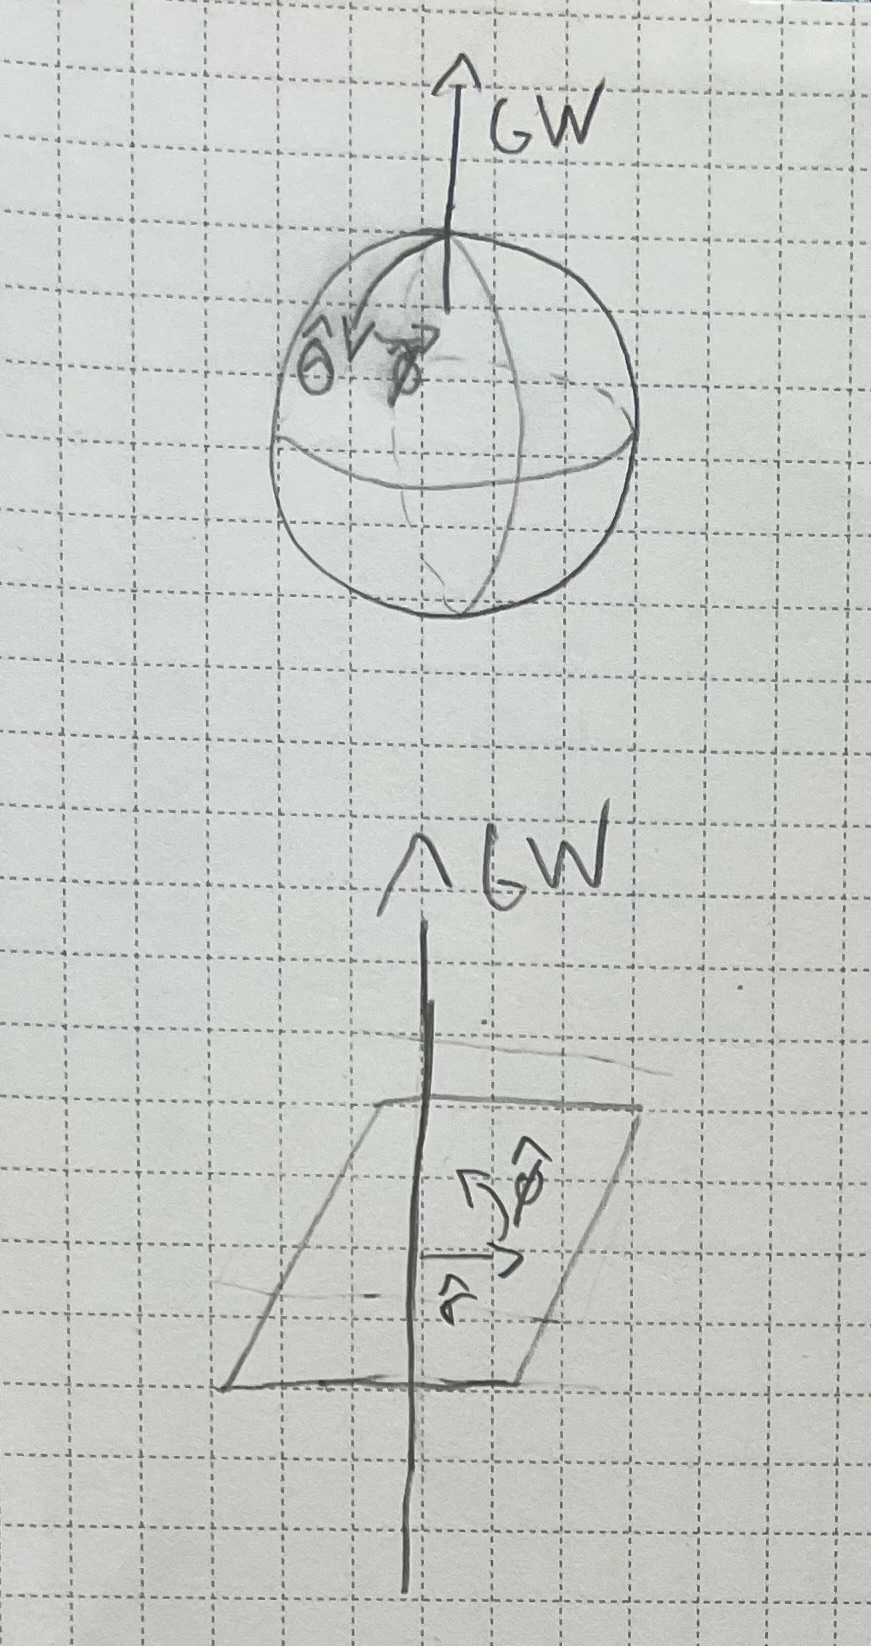
\includegraphics[width=0.25\linewidth]{figures/coord_geometry.jpeg}
    \caption{Unit vectors in relation to a propagating gravitational wave with memory. }
    \label{fig:coord_geometry}
\end{figure}

\section{GW with Memory Statistical Estimate}

%\begin{itemize}
%    \item How many stellar mass BBH mergers are there? How many, how energetic (massive), what is their memory signal time frame? 
%    \item How many supermassive BBH mergers? 
%    \item How many intermediate mass BBH mergers?
%    \item What other memory sources are there? Primordial, re-heating, unbounded (non-linear) BH. 
%\end{itemize}

\subsection{Stellar-mass BBHM}

According to \cite{eldridge2019consistent}, stellar mass black holes (BH) merge with a mean rate density of $\sim$103 Gpc$^{-3}$ yr$^{-1}$ in the local Universe, but there is a large uncertainty and the true value could range from 40 to 213 Gpc$^{-3}$ yr$^{-1}$. For reference the milky way's volume is 509Gpc$^{3}$. This rate was also slightly higher in the early universe (z=3) but drops off exponentially for z higher than 4. Stellar-mass black holes weigh between roughly 5 and 100 solar masses. 
\\

More massive black holes merge less often. Roulet et al. (2020) found that BBHs with a primary mass between 20–30 and a mass ratio $q > 0.5$ at $z \sim 0.2$ have a merger rate of 1.5–5.3 Gpc$^{-3}$ yr$^{-1}$ at the 90\% confidence interval \cite{roulet2020binary}. 
\\

NS–NS (neutron star) and NS–BH binaries are expected to merge at higher rates, 10-1700 and 7.8-140 Gpc$^{-3}$ yr$^{-1}$ \cite{abbott2023population}, respectively, with large uncertainties in large part due to their poorly constrained mass distributions. Merger rates can also be higher by a factor of 10 in the early universe \cite{mandel2022rates}. 
\\

%"the binary black hole merger rate is roughly 50 Gpc$^{-3}$ yr$^{-1}$, or 5 per Myr for a Milky-Way equivalent galaxy with a space density of 0.01 Mpc$^{-3}$" from "Binary evolution via the common-envelope phase" \cite{mandel2022merging}. 
Binary black holes (BBH) with total black-hole mass above roughly 50 solar masses that form due to chemically homogeneous evolution are predicted to have a merger rate of roughly 10 Gpc$^{-3}$ yr$^{-1}$. Current models cannot predict the merger rate for BBHs larger than 50 solar masses. Models suggest that there should be none, but this does not match observational evidence, for example GW190521 \cite{mandel2022merging}. 
\\

The main graphs showing these results is in figures \ref{fig:BBH_mass_dist} and \ref{fig:all_merger_rates}. 

\begin{figure}
    \centering
    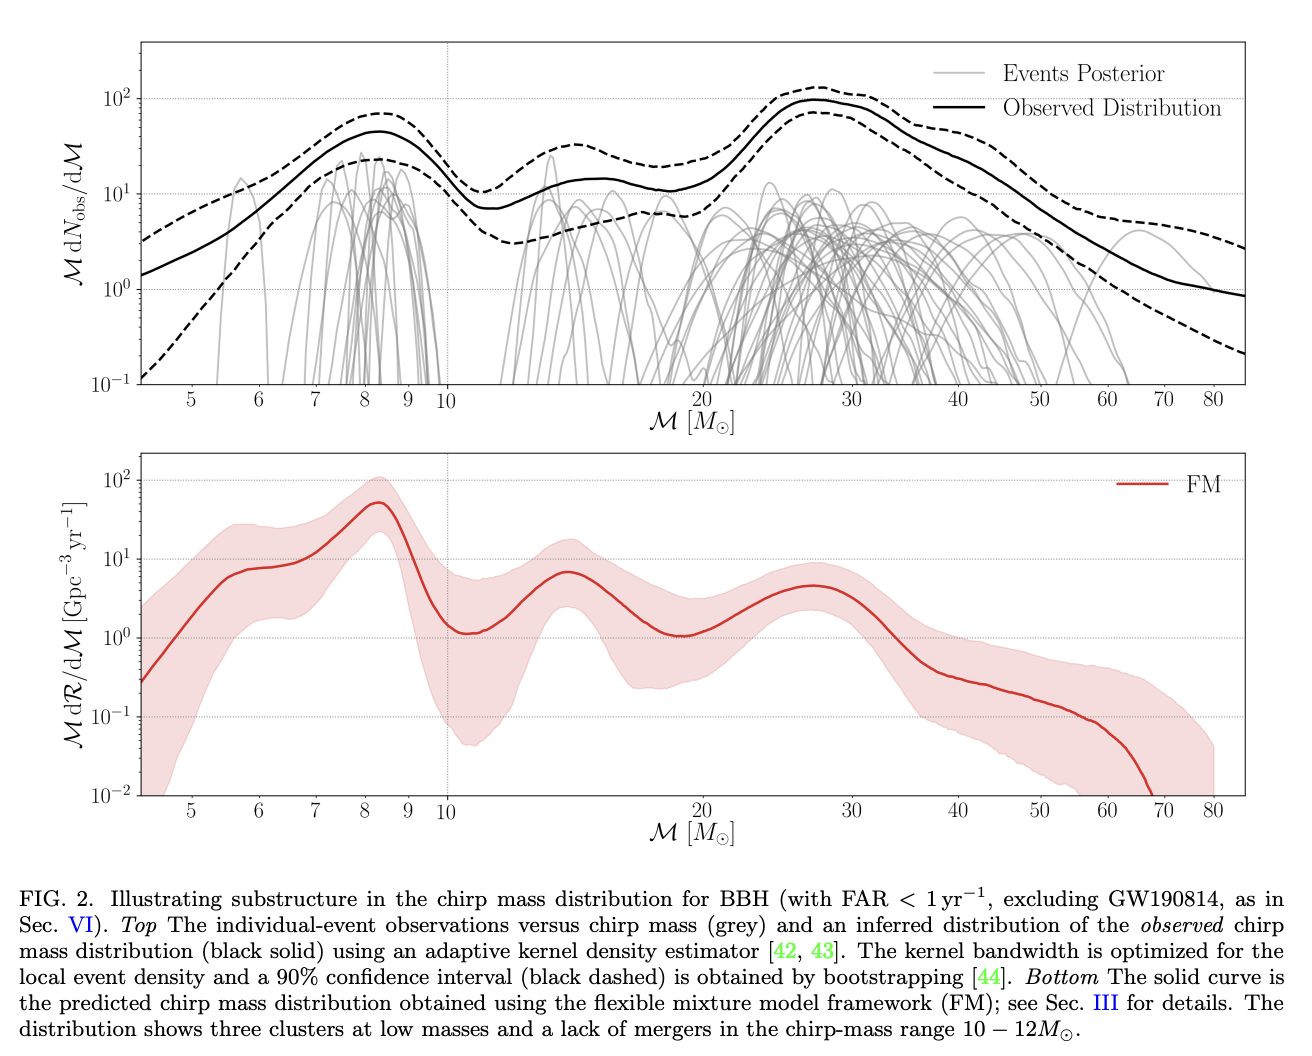
\includegraphics[width=0.8\linewidth]{figures/BBH_mass_dist.png}
    \caption{Stellar mass black hole merger rates vs mass. The predicted (bottom, red) rates do not align with the observed (top, black) rates for massive black holes. Furthermore, with few observations, the observed rates have high error bars. Since this figure is just for reference I copy and pasted their caption without changing it \cite{abbott2023population}.}
    \label{fig:BBH_mass_dist}
\end{figure}


\begin{figure}
    \centering
    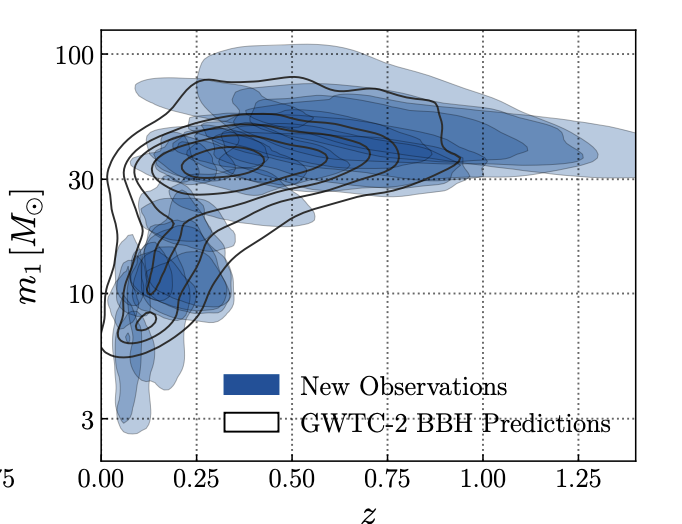
\includegraphics[width=0.5\linewidth]{figures/BBHM_vs_z.png}
    \caption{Observational data from Gravitational Wave Transient Catalog 2 vs predictions \cite{abbott2023population}.}
    \label{fig:BBHM_vs_z}
\end{figure}

\begin{figure}
    \centering
    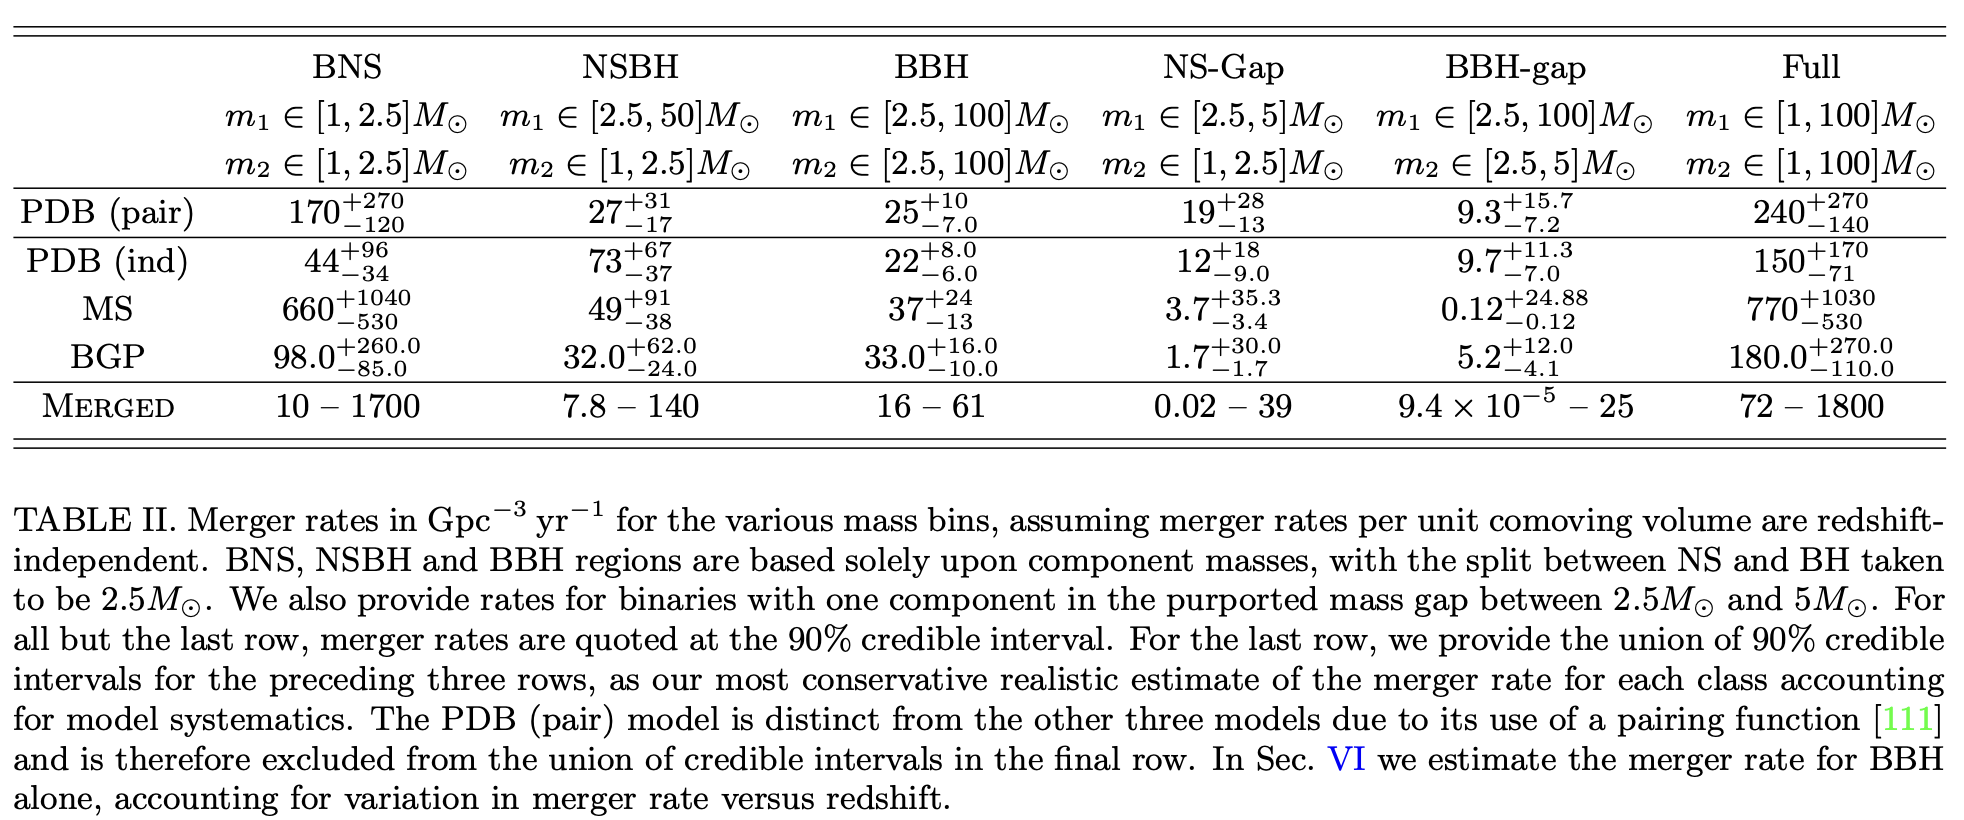
\includegraphics[width=0.7\linewidth]{figures/all_merger_rates.png}
    \caption{Merger rates of Neutron star binaries and neutron stars with stellar mass black holes \cite{abbott2023population}.}
    \label{fig:all_merger_rates}
\end{figure}

\subsection{Supermassive Black Hole Mergers}

There is currently no commonly accepted equation to calculate supermassive black hole merger rates. Erickcek, Kamionkowski, and Benson (2006) reviewed current methods and produced the graph in figure \ref{fig:SMBH_rates}. This paper was produced to predict the merger rates detected by LISA, and therefore only considers supermassive black holes mergers (SMBHM) within LISA's detectable range of $10^4M_\odot$ to $10^8M_\odot$ at $z < 9$. Thankfully, the number of $10^8M_\odot$ black holes exponentially decreases for redshifts larger than 4, so we expect there to be negligibly few $10^8M_\odot$ mergers at $z > 9$. Therefore, this data is a good estimate for all SMBHMs \cite{erickcek2006supermassive}. Figure \ref{fig:SMBH_extra_graphs} shows the uncertainty in SMBHM rates due to unknown cosmological constants and how the rates depend on distance.  
\\

\begin{figure}
    \centering
    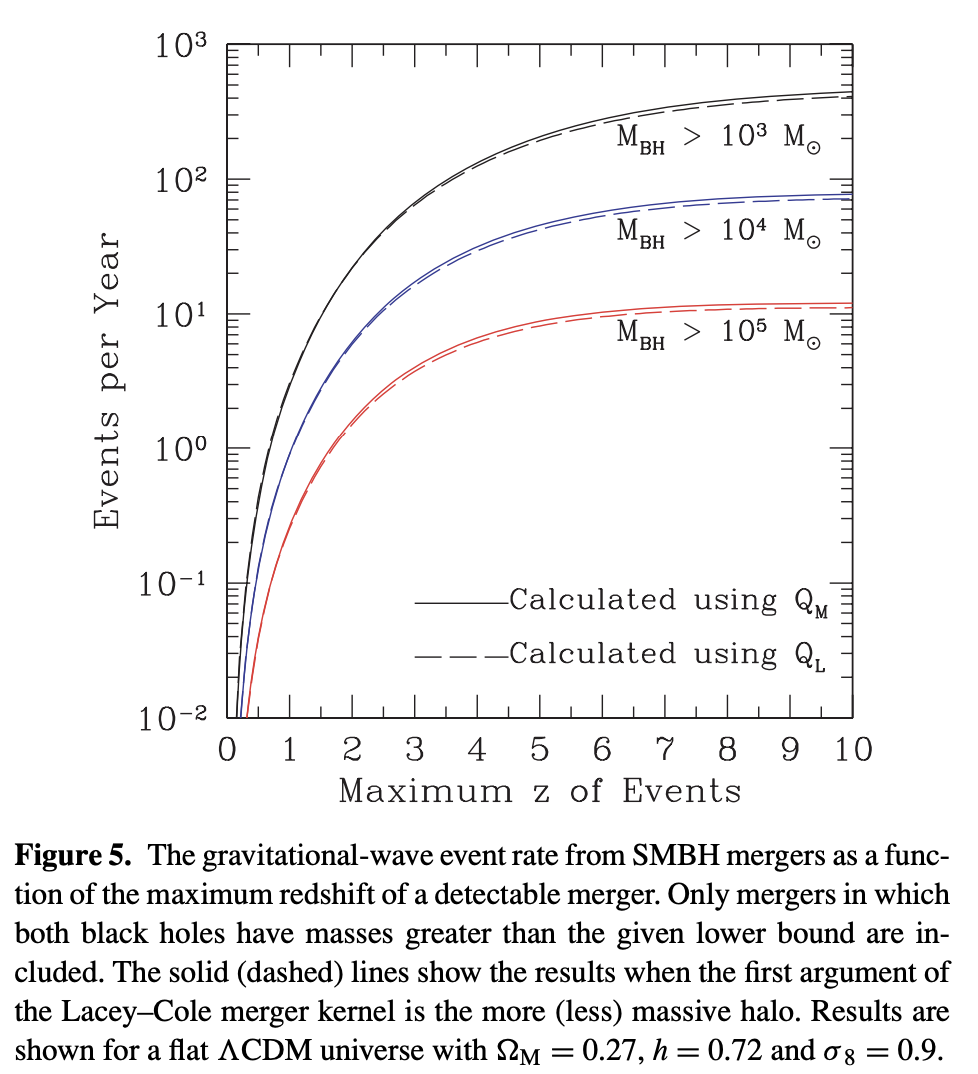
\includegraphics[width=0.5\linewidth]{figures/SMBH_rates.png}
    \caption{Supermassive black hole binary merger rates \cite{erickcek2006supermassive}.}
    \label{fig:SMBH_rates}
\end{figure}

\begin{figure}
    \centering
    \begin{subfigure}[b]{0.45\textwidth}
        \centering
        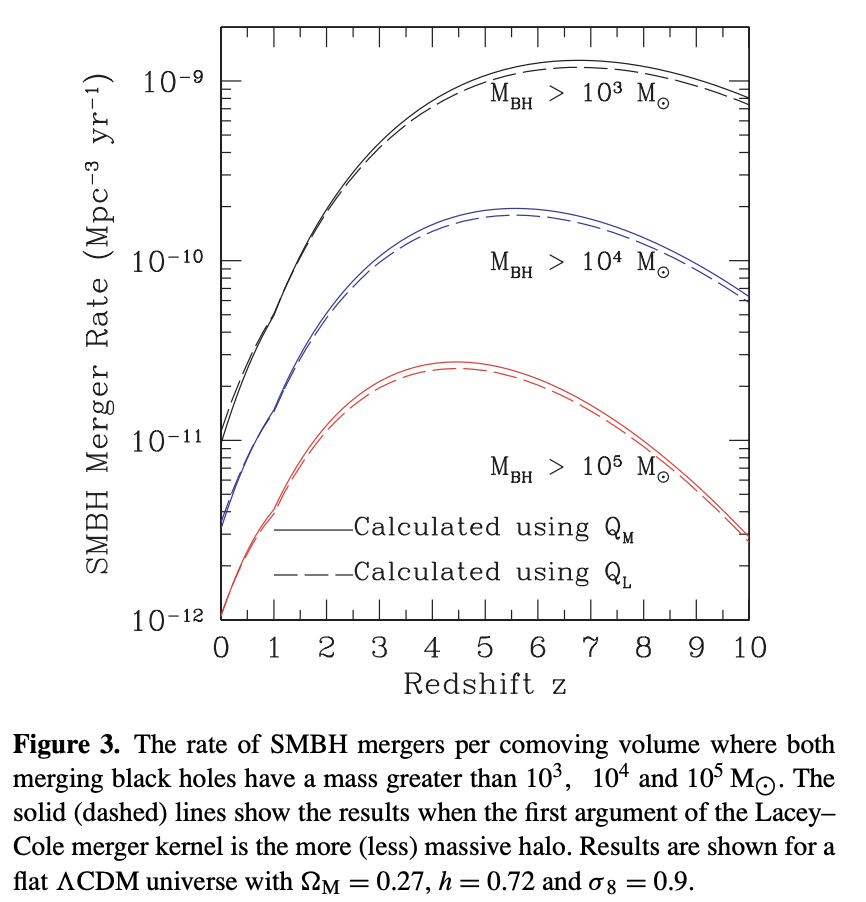
\includegraphics[width=\textwidth]{figures/SMBH_z.png}
        \caption{SMBHM versus redshift \cite{erickcek2006supermassive}.} 
        \label{fig:SMBH_z}
    \end{subfigure}
    \hfill 
    \centering
    \begin{subfigure}[b]{0.45\textwidth}
        \centering
        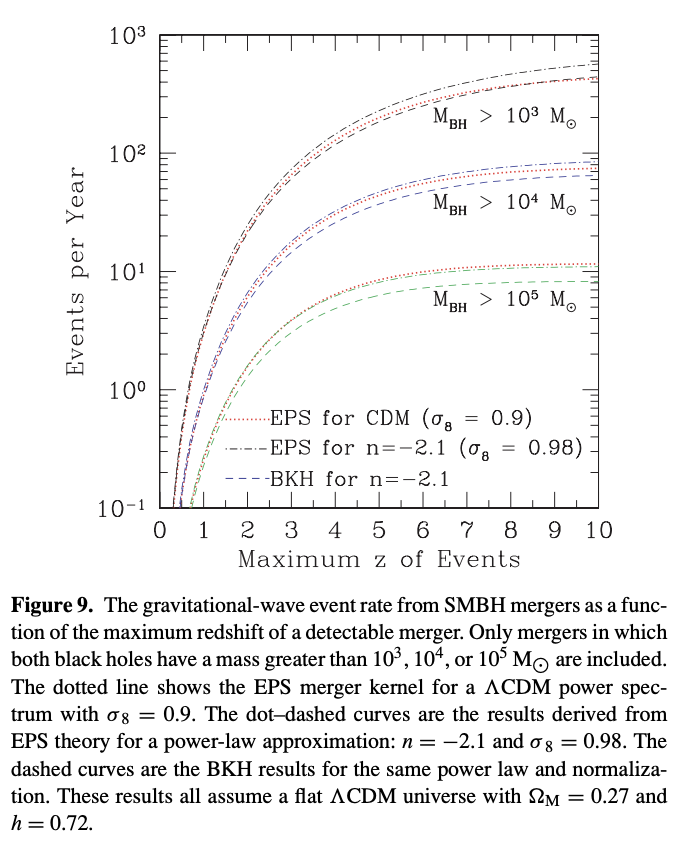
\includegraphics[width=\textwidth]{figures/SMBHM_error.png}
    \caption{Uncertainty in SMBHM rates due to unknown cosmological constants \cite{erickcek2006supermassive}.}
    \label{fig:SMBHM_error}
    \end{subfigure}
    \caption{}
    \label{fig:SMBH_extra_graphs}
\end{figure}

\subsection{Energy Considerations}

Figure \ref{fig:strain_wavelength} shows the characteristic strain amplitude of GWs across the wavelength spectrum. 

\begin{figure}
    \centering
    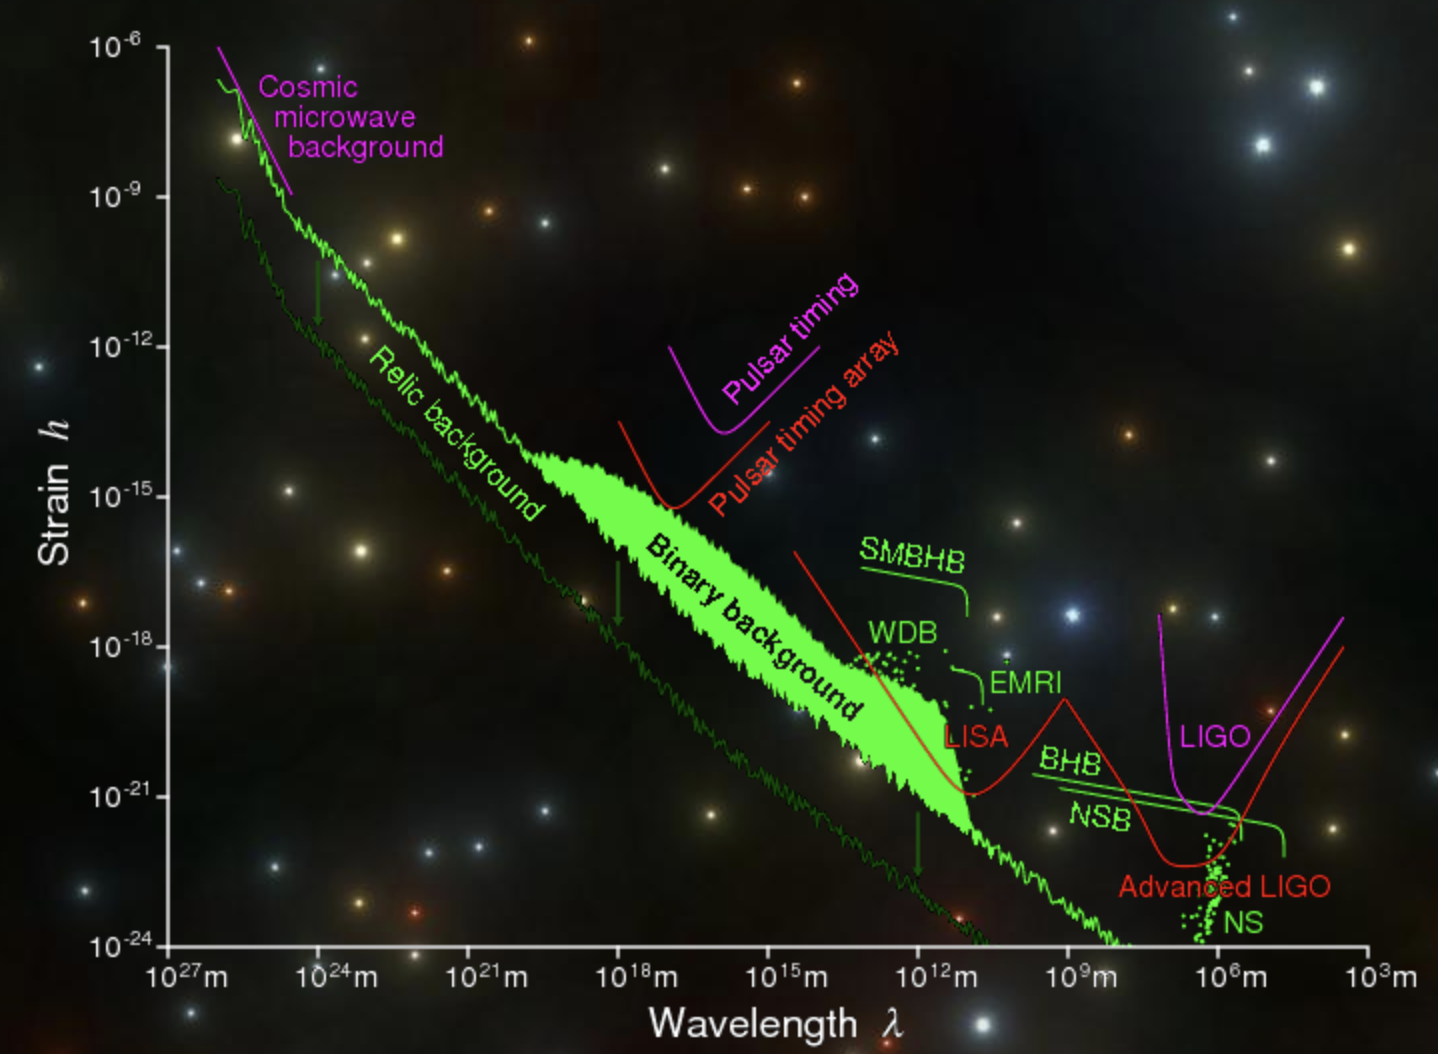
\includegraphics[width=0.5\linewidth]{figures/strain_wavelength.png}
    \caption{Characteristic strain vs GW wavelength from \hyperlink{http://www.tapir.caltech.edu/~teviet/Waves/gwave_spectrum.html}{caltech.edu}.}
    \label{fig:strain_wavelength}
\end{figure}

\begin{figure}
    \centering
    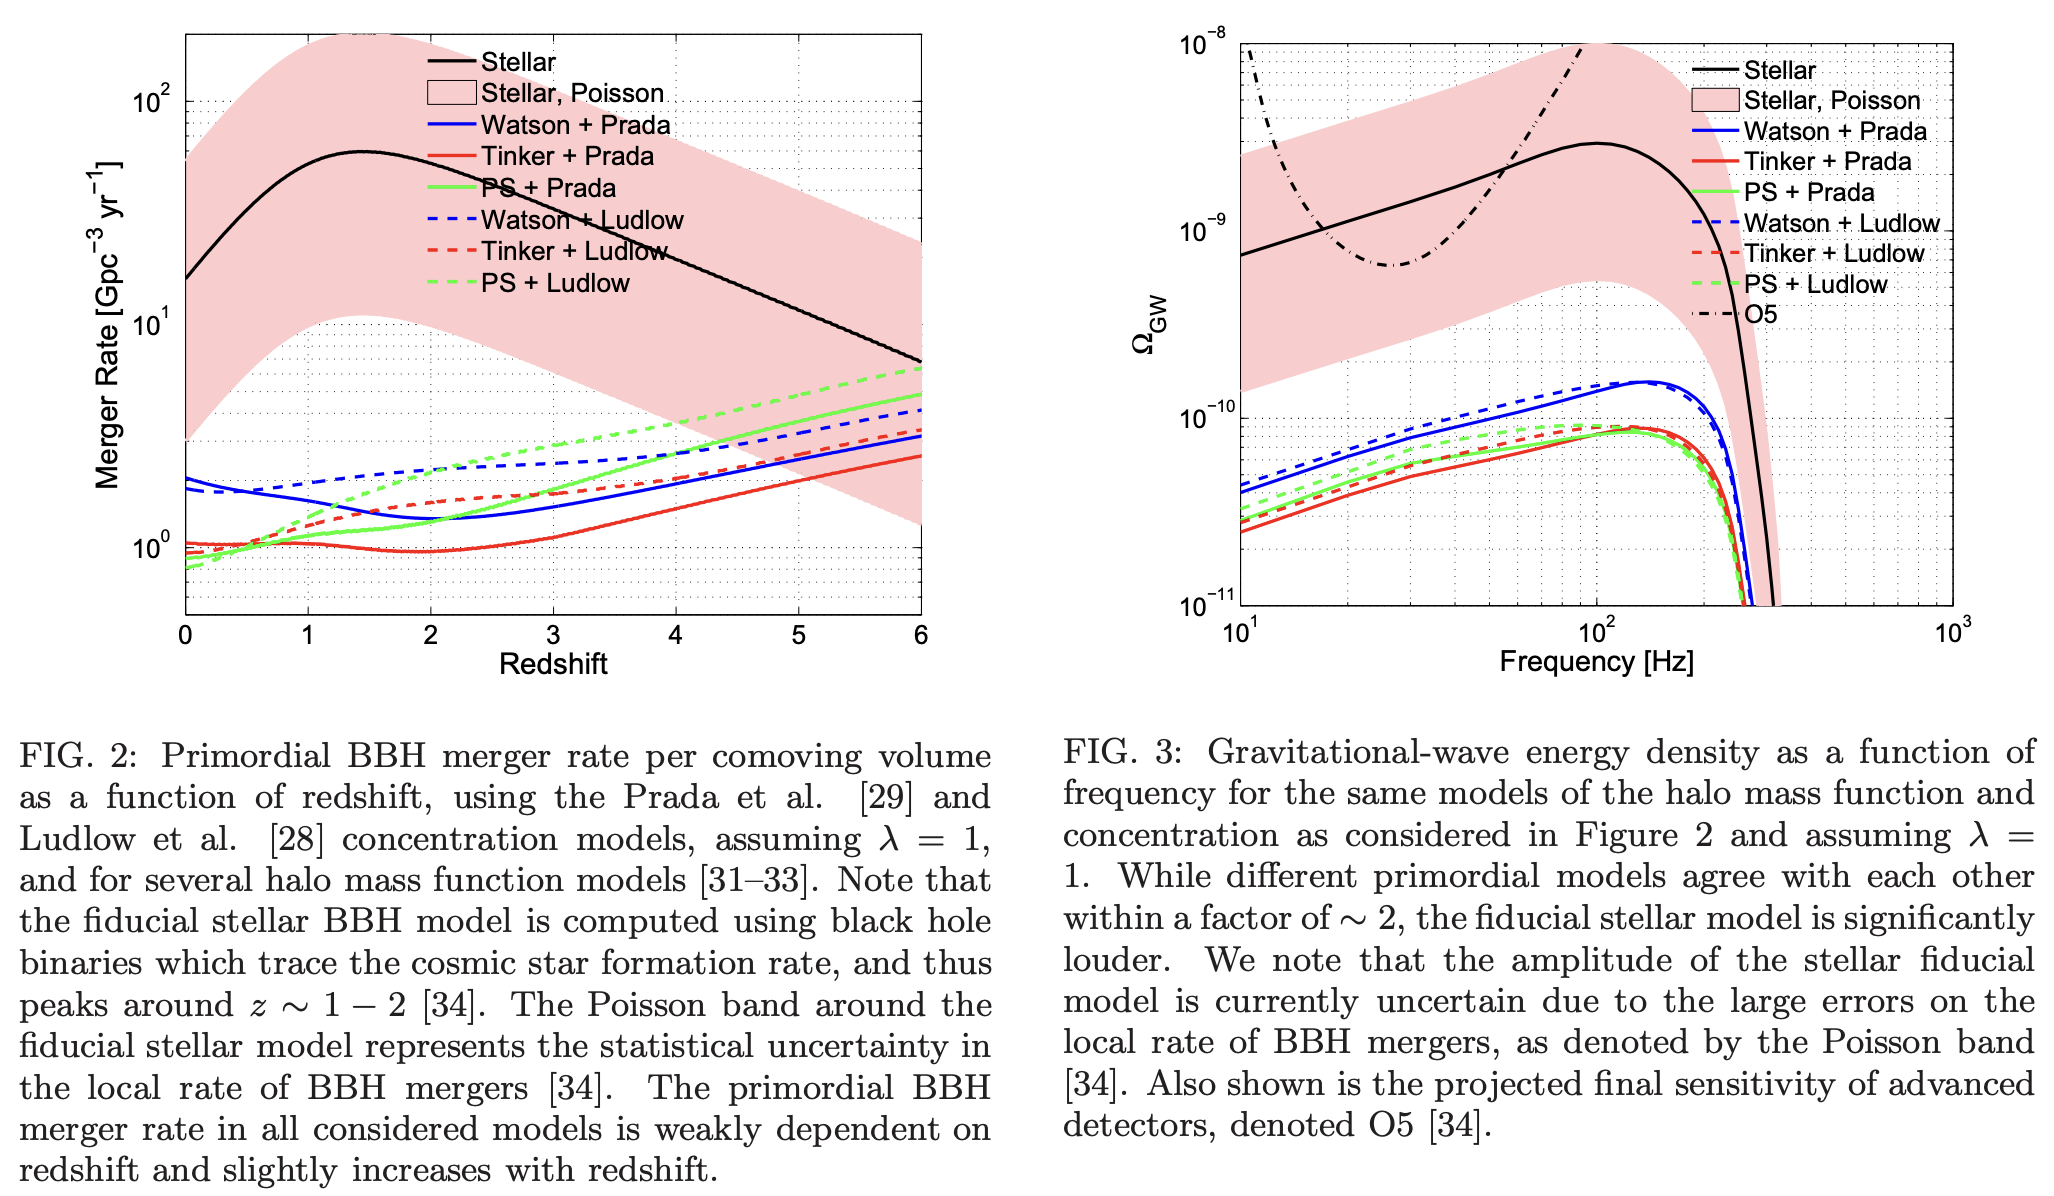
\includegraphics[width=0.85\linewidth]{figures/BBH energy density per Hz.png}
    \caption{}
    \label{fig:BBH energy density per Hz}
\end{figure}


\subsection{Other Sources: Primordial GWs, re-heating, unbounded (non-linear) orbits}

\subsection{Instrumentation}

Atacama Cosmology Telescope (ACT) produces arcminute-resolution and micro-Kelvin sensitivity maps of the CMB over 200 square degree of the sky in three frequency bands \cite{kosowsky2003atacama}. Aiola et al (2020) used ACT data to cover a map of over 17,000 deg$^2$, and it has a 1 degree field of view. 
\\

The South Pole Telescope (SPT-3G) has a field of view of 1 degree \cite{ruhl2004south}. 


\newpage
\printbibliography
\end{document}